\documentclass[tikz, border=4pt]{standalone}
\usepackage{tikz}
\usepackage{karnaugh-map}
\begin{document}
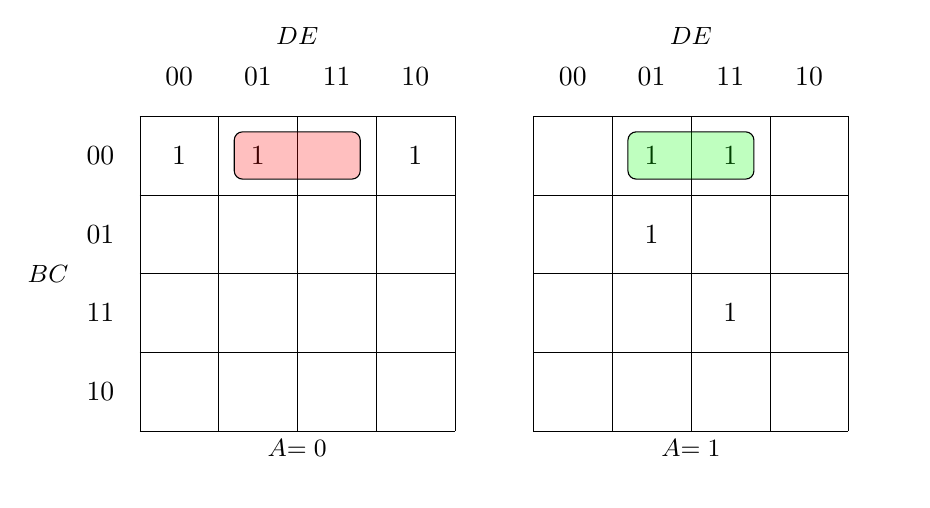
\begin{tikzpicture}[x=1cm, y=1cm]
  \node[inner sep=0pt] at (5.78,-3.11) {\pgfinterruptpicture%
  \begin{karnaugh-map}[4][4][2][$E$][$D$][$C$][$B$][$A$]
    \minterms{0,1,2,17,19,21,31}
    \implicant{1}{3}
    \implicant{1}{3}[1]
  \end{karnaugh-map}%
  \endpgfinterruptpicture};
\end{tikzpicture}
\end{document}
